% Auto-generated from committed gate JSONs by generate_figures.py. Do not edit by hand.

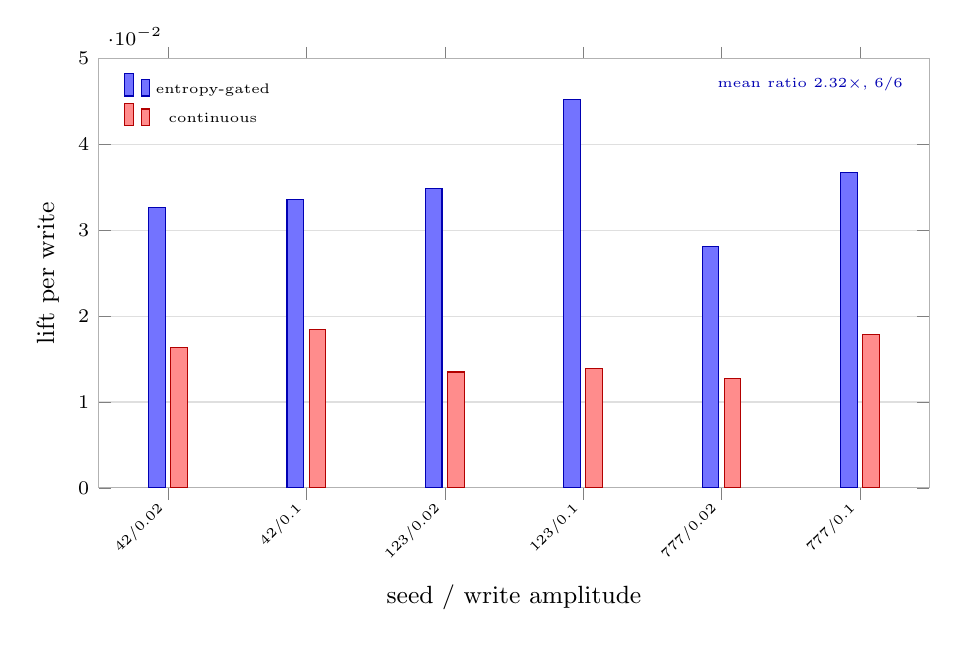
\begin{tikzpicture}
\begin{axis}[
  ybar, /pgf/bar width=6pt,
  width=\columnwidth, height=0.58\columnwidth,
  symbolic x coords={42/0.02,42/0.1,123/0.02,123/0.1,777/0.02,777/0.1},
  xtick=data, x tick label style={rotate=45, anchor=east, font=\tiny},
  xlabel={seed / write amplitude}, xlabel style={font=\scriptsize},
  ymin=0, ymax=0.05, ylabel={lift per write},
  label style={font=\small}, tick label style={font=\scriptsize},
  legend style={font=\tiny, at={(0.02,0.98)}, anchor=north west, draw=none, fill=none},
  ymajorgrids, grid style={gray!25}, axis line style={gray!60},
]
\addplot+[fill=blue!55, draw=blue!70!black] coordinates {(42/0.02,0.0327) (42/0.1,0.0336) (123/0.02,0.0349) (123/0.1,0.0452) (777/0.02,0.0281) (777/0.1,0.0367)};
\addplot+[fill=red!45, draw=red!70!black] coordinates {(42/0.02,0.0164) (42/0.1,0.0184) (123/0.02,0.0135) (123/0.1,0.0139) (777/0.02,0.0127) (777/0.1,0.0179)};
\addlegendentry{entropy-gated}
\addlegendentry{continuous}
\node[font=\tiny, blue!70!black, anchor=north east] at (rel axis cs:0.98,0.98)
  {mean ratio 2.32$\times$, 6/6};
\end{axis}
\end{tikzpicture}
